% 18 variables in here:
% h_1 = 10.0, h_2 = 10.0, h_3 = 10.0, h_4 = 10.0, h_5 = 10.0, h_6 = 10.0, ux_1 = 0.0, ux_2 = 0.0, ux_3 = 0.0, ux_4 = 0.0, ux_5 = 0.0, ux_6 = 0.0, uy_1 = 0.0, uy_2 = 0.0, uy_3 = 0.0, uy_4 = 0.0, uy_5 = 0.0, uy_6 = 0.0
\begin{figure}[ht!]
\centering
  % \quad \subfloat[$SE^1_x$] {
  %   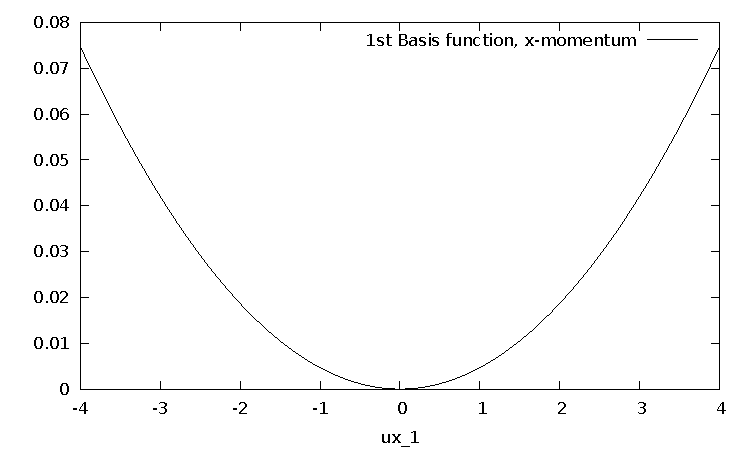
\includegraphics[scale=\zoomfactor]{{{ord2_varying_ux_1/10.0_10.0_10.0_10.0_10.0_10.0_y_0.0_0.0_0.0_0.0_0.0_0.0_0.0_0.0_0.0_0.0_0.0f00}}}
  % }
  % \quad \subfloat[] {
  %   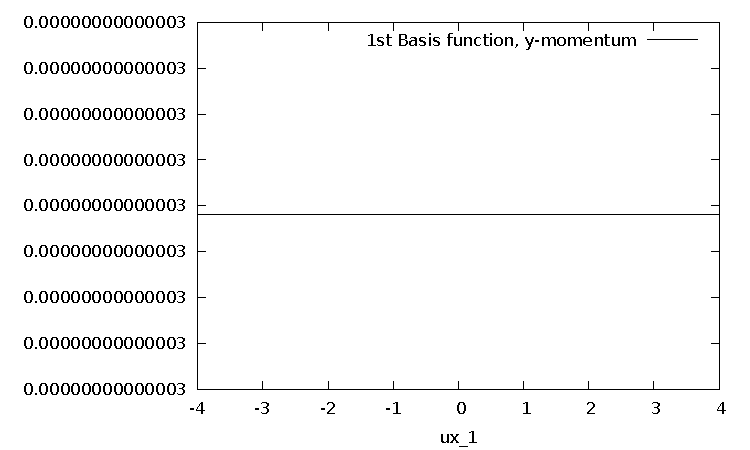
\includegraphics[scale=\zoomfactor]{{{ord2_varying_ux_1/10.0_10.0_10.0_10.0_10.0_10.0_y_0.0_0.0_0.0_0.0_0.0_0.0_0.0_0.0_0.0_0.0_0.0f01}}}
  % }
  \quad \subfloat[$SE^2_x$. $SE^1_x$, $SE^3_x$, $SE^4_x$, $SE^6_x$ are very similar in shape, but all smaller than $SE_x^2$.] {
    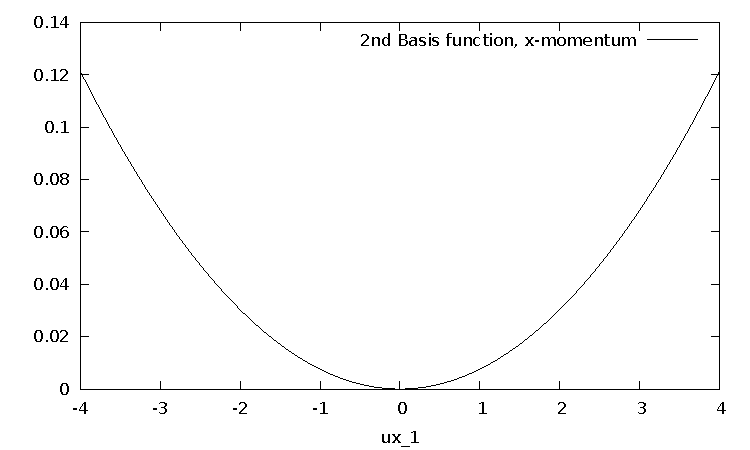
\includegraphics[scale=\zoomfactor]{{{ord2_varying_ux_1/10.0_10.0_10.0_10.0_10.0_10.0_y_0.0_0.0_0.0_0.0_0.0_0.0_0.0_0.0_0.0_0.0_0.0f02}}}
  }
  % \quad \subfloat[] {
  %   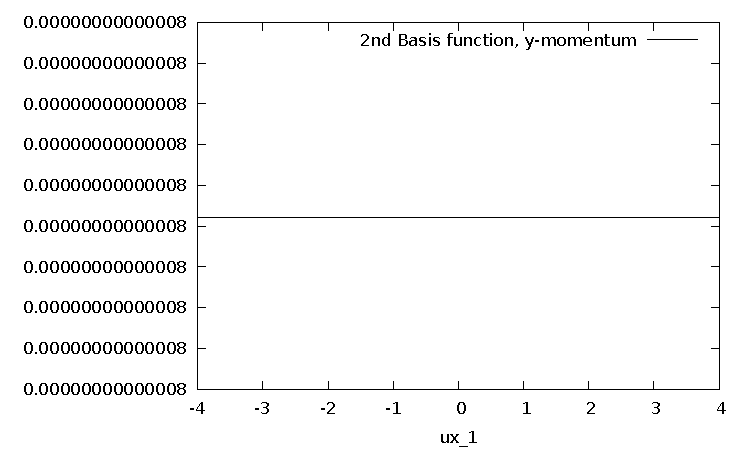
\includegraphics[scale=\zoomfactor]{{{ord2_varying_ux_1/10.0_10.0_10.0_10.0_10.0_10.0_y_0.0_0.0_0.0_0.0_0.0_0.0_0.0_0.0_0.0_0.0_0.0f03}}}
  % }
  % \quad \subfloat[$SE^3_x$] {
  %   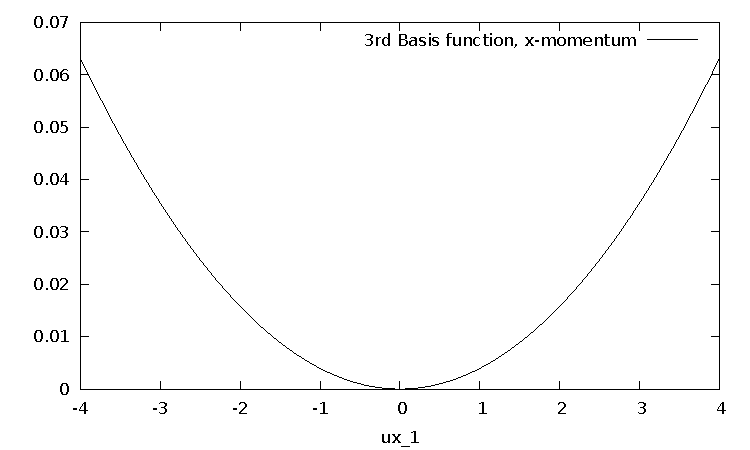
\includegraphics[scale=\zoomfactor]{{{ord2_varying_ux_1/10.0_10.0_10.0_10.0_10.0_10.0_y_0.0_0.0_0.0_0.0_0.0_0.0_0.0_0.0_0.0_0.0_0.0f04}}}
  % }
  % \quad \subfloat[] {
  %   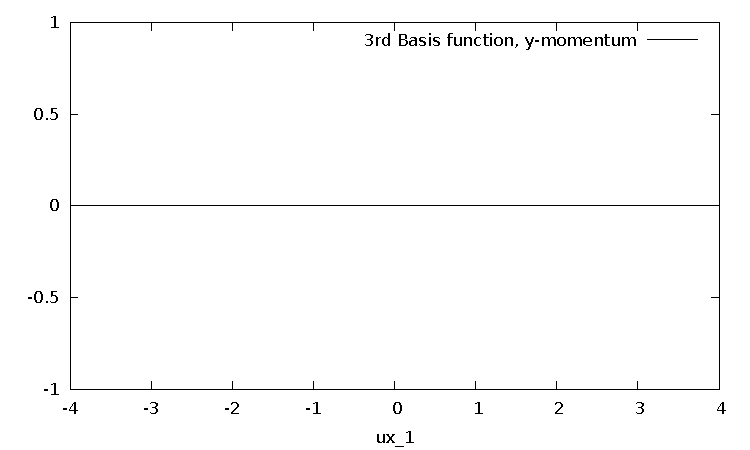
\includegraphics[scale=\zoomfactor]{{{ord2_varying_ux_1/10.0_10.0_10.0_10.0_10.0_10.0_y_0.0_0.0_0.0_0.0_0.0_0.0_0.0_0.0_0.0_0.0_0.0f05}}}
  % }
  % \quad \subfloat[$SE^4_x$] {
  %   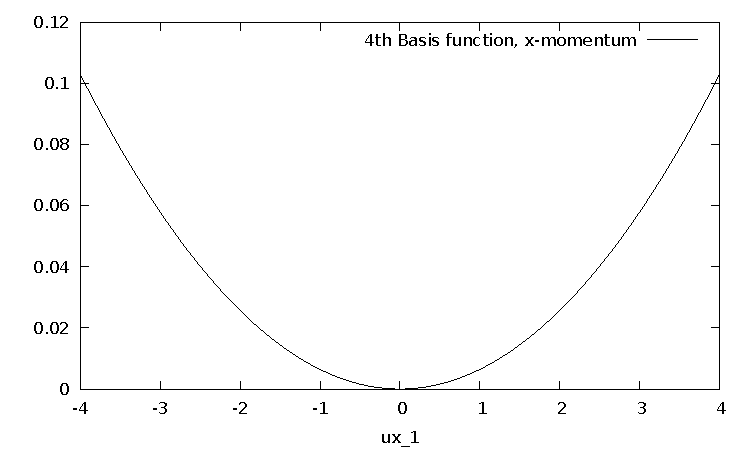
\includegraphics[scale=\zoomfactor]{{{ord2_varying_ux_1/10.0_10.0_10.0_10.0_10.0_10.0_y_0.0_0.0_0.0_0.0_0.0_0.0_0.0_0.0_0.0_0.0_0.0f06}}}
  % }
  % \quad \subfloat[] {
  %   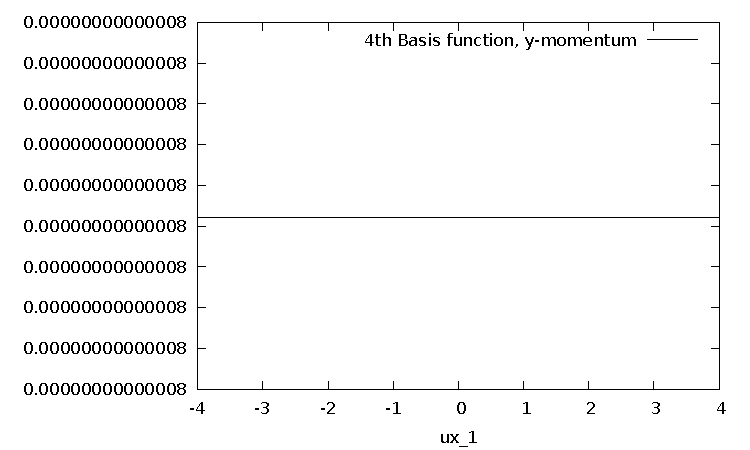
\includegraphics[scale=\zoomfactor]{{{ord2_varying_ux_1/10.0_10.0_10.0_10.0_10.0_10.0_y_0.0_0.0_0.0_0.0_0.0_0.0_0.0_0.0_0.0_0.0_0.0f07}}}
  % }
  \quad \subfloat[$SE^5_x$, $SE_y^i$ for all basis functions] {
    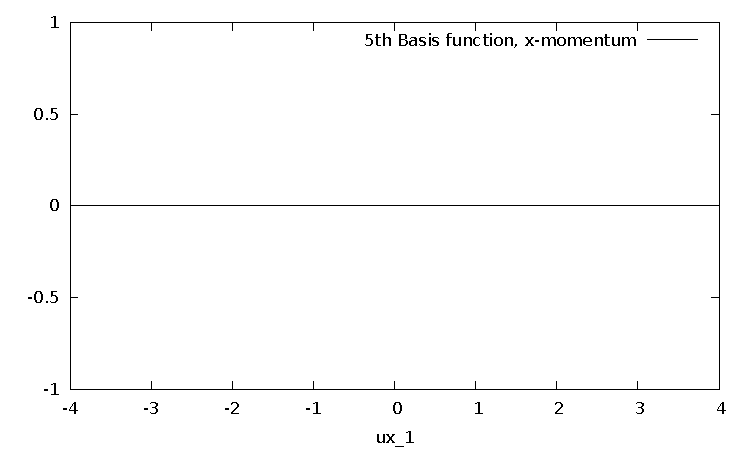
\includegraphics[scale=\zoomfactor]{{{ord2_varying_ux_1/10.0_10.0_10.0_10.0_10.0_10.0_y_0.0_0.0_0.0_0.0_0.0_0.0_0.0_0.0_0.0_0.0_0.0f08}}}
  }
  % \quad \subfloat[] {
  %   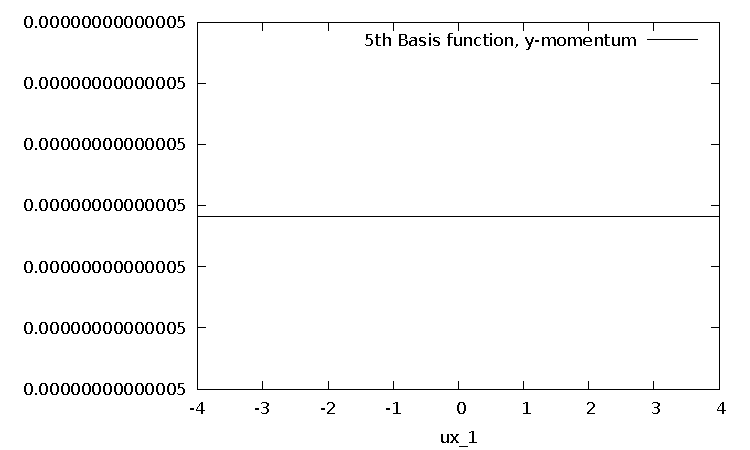
\includegraphics[scale=\zoomfactor]{{{ord2_varying_ux_1/10.0_10.0_10.0_10.0_10.0_10.0_y_0.0_0.0_0.0_0.0_0.0_0.0_0.0_0.0_0.0_0.0_0.0f09}}}
  % }
  % \quad \subfloat[$SE^6_x$] {
  %   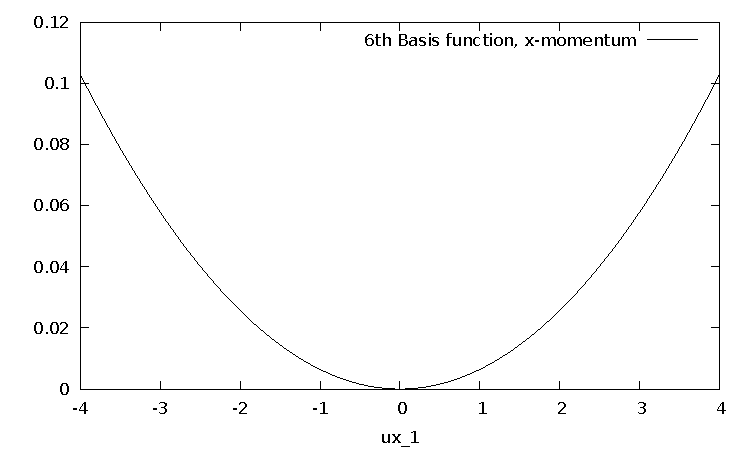
\includegraphics[scale=\zoomfactor]{{{ord2_varying_ux_1/10.0_10.0_10.0_10.0_10.0_10.0_y_0.0_0.0_0.0_0.0_0.0_0.0_0.0_0.0_0.0_0.0_0.0f10}}}
  % }
  % \quad \subfloat[] {
  %   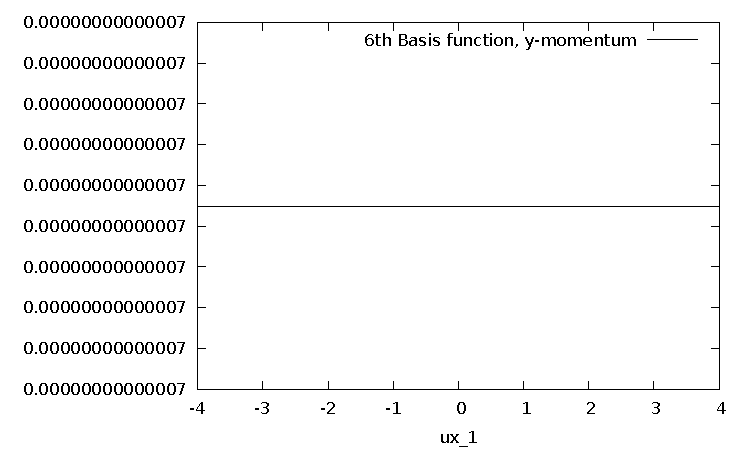
\includegraphics[scale=\zoomfactor]{{{ord2_varying_ux_1/10.0_10.0_10.0_10.0_10.0_10.0_y_0.0_0.0_0.0_0.0_0.0_0.0_0.0_0.0_0.0_0.0_0.0f11}}}
  % }
\caption{Error plots for varying $u_{x,1}$. All other momentums are set to 0 (i.e. $u_{x,2}=\dots=u_{x,6}=u_{y,1}=\dots=u_{y,6}=0$), all heights are set to 10 (i.e. $h_1=\dots=h_6=10$). The error is zero for \emph{all} $y$-momentums and for the $x$-momentum of the 5th basis function. 
%$SE_x^5$ and all $SE_y^i$ are omitted since they are 0 within the whole range.
}
\label{fig:ord2_varying_ux_1}
\end{figure}

%%% Local Variables:
%%% TeX-master: "../results.tex"
%%% End:
